\section{Basics}

\subsection{Digital Signal Processing}

\subsubsection{Digital Filters}

\subsubsubsection{Finite Impulse Response Filter}

Digital Filters are a huge field of digital signal processing. The most common filters are \ac{FIR}-filters.
These are also called \frqq non-recursive filters\flqq .
The basic structure is a weighted shift register without feedback. The missing feedback is what makes
the \ac{FIR}-filter stable per construction.

In \autoref{fig:FIR-filter} the structure of a \ac{FIR}-filter is shown.

\begin{figure}[!h]
    \centering
    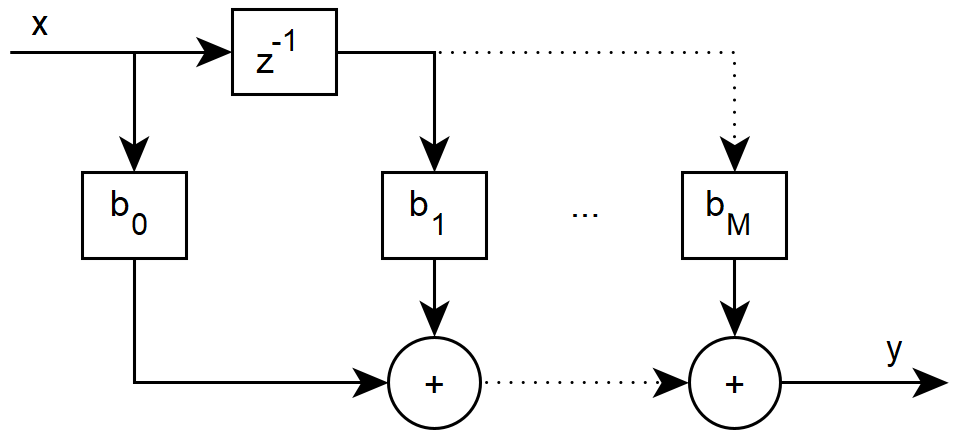
\includegraphics[width=7cm]{img/fir.png}
    \caption{Basic structure of a $M$ order \ac{FIR}-filter in the first canonical form \cite{meyer_signalverarbeitung}}
    \label{fig:FIR-filter}
\end{figure}

It can be seen that there are multiple components in this filter. The first component is the delay block,
which is described as $z^{-1}$. This block is responsible for adding a delay of one clock cycle to the input data.
Secondly, there are multiplication blocks, noted as $b_M$. These blocks weight the input data and give the
result to an adder, which adds $M+1$ weighted and delayed signal samples. This sum is the output of an
\ac{FIR}-filter. It also means, that the output is only dependend on the present and the $M$ last input samples
and not of the past output.

The input signal is $x$, whereas the output is $y$. The order of this Filter is $M$ which means the amount of
filter taps or delay blocks.

A special case of the \ac{FIR}-filter is the \textit{Moving Average Filter}, at which all coefficients are $\frac{1}{M+1}$.

The whole system can be described with the difference equation in the time-domain (\autoref{eq:fir-difference-eq})

\begin{equation}
    y[n] = b_0 \cdot x[n] + b_1 \cdot x[n-1] + ... + b_M \cdot x[n-M]
    \label{eq:fir-difference-eq}
\end{equation},

or with the transfer function in the z-domain (\autoref{eq:fir-transfer-func})

\begin{equation}
    H(z) = b_0 + b_1 \cdot z^{-1} + ... + b_M \cdot z^{-M}
    \label{eq:fir-transfer-func}
\end{equation}.

The output can be calculated with the convolution (noted as $*$) of the impulse response $h[n]$, which is simply the
union of the filter coefficients, and the input signal $x[n]$ (\autoref{eq:conv}).

\begin{equation}
    y[n] = x[n] * h[n]
    \label{eq:conv}
\end{equation}

Another way to describe the filtering result is in the frequency domain.
If the frequency of the input is given with $X(z)$ and the frequency response of the filter is $H(z)$
than the output is $Y(z)$, which can be calculated like shown in \autoref{eq:freq-response}.

\begin{equation}
    Y(z) = X(z) \cdot H(z)
    \label{eq:freq-response}
\end{equation}

The stability of the \ac{FIR}-filter is characteristic, this can be seen in the pole-zero plane. All poles are in
the middle of the unit circle, which is necessary for the stability of a system.

If the value of the z-plane is evaluated on the unit circle the result is the frequency response of the filter
(\autoref{fig:FIR-z-plane-and-freq}).

\begin{figure}[!h]
    \begin{subfigure}[c]{0.35\textwidth}
        \centering
        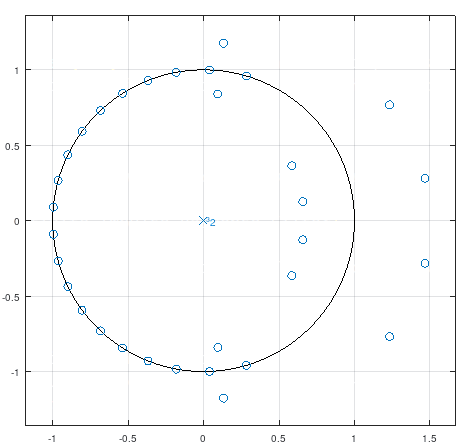
\includegraphics[width=\textwidth]{img/fir-zplane.png}
    \end{subfigure}
    \begin{subfigure}[c]{0.65\textwidth}
        \centering
        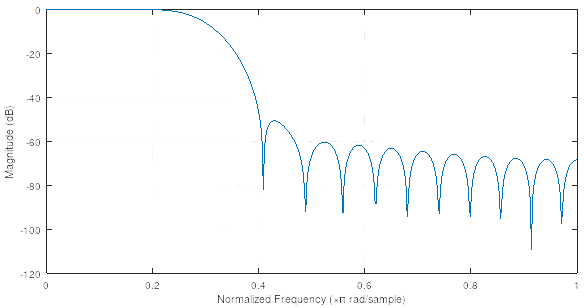
\includegraphics[width=\textwidth]{img/fir-freq.png}
    \end{subfigure}
    \caption{z-plane plot (left) and frequency response (right) of a \ac{FIR}-lowpass-filter}
    \label{fig:FIR-z-plane-and-freq}
\end{figure}

\subsubsubsection{Infinite Impulse Response Filter}

Another filter type is the \ac{IIR} filter. The structure is recursive as it is shown in \autoref{fig:IIR-filter}.

\begin{figure}[!h]
    \centering
    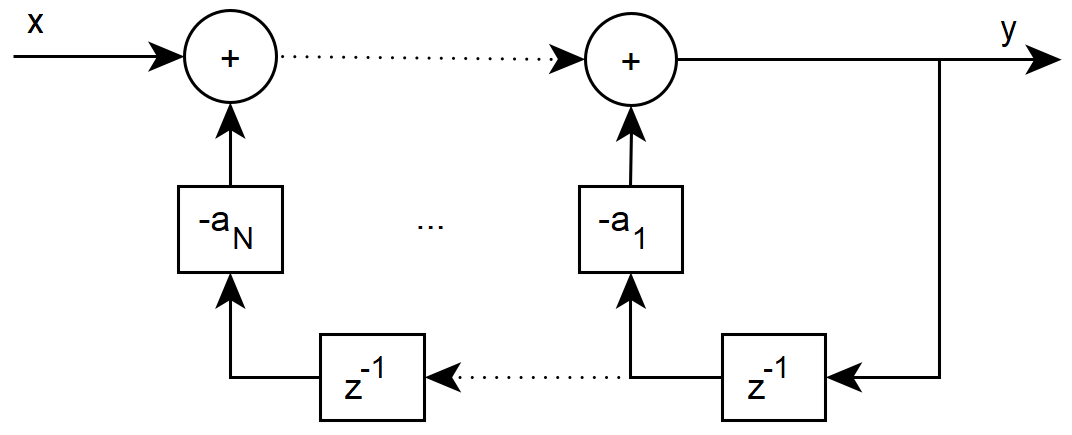
\includegraphics[width=7cm]{img/iir.png}
    \caption{Basic structure of a $M$ order \ac{IIR}-filter in the first canonical form \cite{meyer_signalverarbeitung}}
    \label{fig:IIR-filter}
\end{figure}

Due to this recursive structure, this type of filter is no longer necessarilly stable. This means, that it can
oscillate and possibly the output can grow exponentially. To fulfill stability, all the poles of the
\ac{IIR}-filter have to be in the unit-circle \cite{meyer_signalverarbeitung}.

Its transfer function can be described as follows:

\begin{align}
    H(z) = \frac{1}{a_1 \cdot z^{-1} + ... + a_M \cdot z^{-M}}
\end{align}

In the time domain, the output is equal to

\begin{align}
    y[n] = x[n] - a_1 \cdot y[n-1] - a_2 \cdot y[n-2] - ... - a_M \cdot y[n-M]
\end{align}
.

The output is dependend on the current signal and all the $M$ outputs before. In literature and other documentation,
the $a_0$-coefficient is also referenced. This is the amplification of the output signal. Due to filter-stability-reasons,
this coefficient is typically set to $1$ \cite{arm_dsp} \cite{cookbook_audio}.

If the two types of filters are getting merged, the result is also an \ac{IIR}-filter, plus
a few additional feed-forward-terms. A widely used example of this is the \textit{Biquad-filter} \cite{arm_dsp}.

These filters use two filter-taps in the forward- and two taps in the feedback-path. The structure
is shown in \autoref{fig:biquad-structure}.

\begin{figure}[!h]
    \centering
    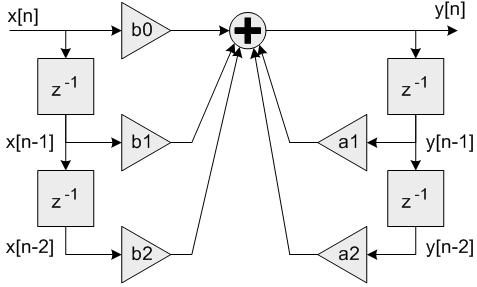
\includegraphics[width=7cm]{img/biquad_structure.png}
    \caption{Structure of a biquad filter \cite{arm_dsp}}
    \label{fig:biquad-structure}
\end{figure}

The transfer function of this filtertype is:

\begin{align}
    H(z) = \frac{b_0 + b_1 \cdot z^{-1} + b_2 \cdot z^{-2}}{a_1 \cdot z^{-1} + a_2 \cdot z^{-2}}
\end{align}

Here it can be seen, why this filter is called \frqq biquad\flqq{}: it is the short form for
\frqq bi-quadratic\flqq{}, which relates to the powers of the numerator- and denominator-terms.
Also in this structure, the $a_0$-coefficient is set to $1$.

This transfer function leeds to an output of:

\begin{align}
    y[n] = b_0 \cdot x[n] + b_1 \cdot x[n-1] + b_2 \cdot x[n-2] - a_1 \cdot y[n-1] - a_2 \cdot y[n-2]
\end{align}

It is worth noting, that the denominator-coefficients have to be negated to match the structure in
\autoref{fig:biquad-structure}.


\subsubsubsection{Filter Design}

This section deals with designing filters. There are a few ways to calculate the numerator and
denominator-coefficients. But this shouldn't be part of this section, the goal is more like looking at
how to design a filter in a high-level perspective.

First of all, the number of filtertaps will be discussed. As stated earlier, \ac{FIR}-filters have
the convenient property, that they are always stable. The downside of these filters are,
that for example a narrow-band bandpass filter needs more filtertaps, than a comparable
\ac{IIR}-filter \cite{meyer_signalverarbeitung}. This should not be a huge problem in the most cases,
but if the goal is to variate the filter-coefficients, this may lead to problems. Additionally, a longer filter
could leed to a bigger latency.

Secondly, the shape of \ac{FIR} and \ac{IIR}-filters differ. The recursive filter is more often used to
model an actual analog filter \cite{meyer_signalverarbeitung}.

In the following graphics, there is a \ac{FIR}- on the left and a \ac{IIR}-bandpass-filter on the right.
All the parameters of these two filters, mid-frequency, bandwidth, quality-factor and number of coefficients
are set equal in order to make them comparable.

\begin{figure}[!h]
    \centering
    \begin{subfigure}[c]{0.49\textwidth}
        \centering
        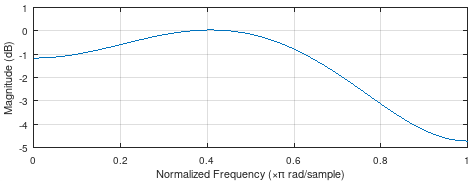
\includegraphics[width=\textwidth]{img/fir_bandpass.png}
    \end{subfigure}
    \begin{subfigure}[c]{0.49\textwidth}
        \centering
        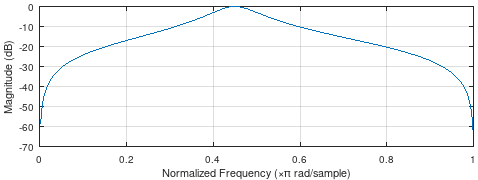
\includegraphics[width=\textwidth]{img/iir_bandpass.png}
    \end{subfigure}
    \caption{Comparison of the frequency response of a \ac{FIR}- (left) and \ac{IIR}-bandpass-filter (right)}
    \label{fig:fir-iir-compare}
\end{figure}

The parameters which were chosen for this comparison were set to:

\begin{table}[!h]
    \centering
    \caption{Parameters to compare \ac{FIR}- and \ac{IIR}-filters}
    \label{table:compare-filters}
    \begin{tabular}{c | c | c }
        start-frequency & stop-frequency & number of coefficients \\
        \hline
        0.4 & 0.5 & 5
    \end{tabular}
\end{table}

As it can be observed, the \ac{IIR}-filter has much sharper edges and the attenuation in the stopband is much higher.
This is due to the fact, that \ac{IIR}-filters have poles, which can produce sharper edges, but it can also lead to
instability.

As a reference, an analog bandpass-filter is shown in \autoref{fig:analog-bandpass}, designed with the Texas Instruments
filter-design-tool \cite{TI-filterdesign-tool}.

\begin{figure}[!h]
    \centering
    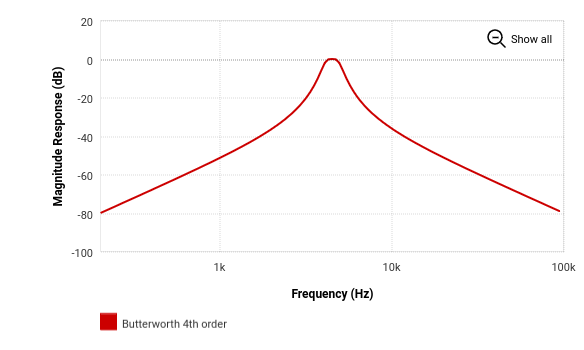
\includegraphics[width=8cm]{img/analog_bandpass.png}
    \caption{Analog bandpass filter frequency response}
    \label{fig:analog-bandpass}
\end{figure}

It can be seen, that the basic shape of the \ac{IIR}-filter is much closer to the analog equivalent than the
\ac{FIR}-filter.

\subsection{Microcontroller-Peripherals}

\subsubsection{Inter-Integrated Sound}

The \ac{I2S} protocol was developed by \textit{Philips} to share audio between \acp{IC}.
A similarity to the \ac{SPI} protocol can be recognized.

There are three signal lines:
\begin{itemize}
    \item SCK: Clock signal
    \item SD: Data signal
    \item WS: Word select, for distinction between left and right channel
\end{itemize}
So the data is transmitted over the same signal line by time division multiplexing. 
To illsutrate the timing of the protocol the corresponding diagrams are shown in \autoref{fig:i2s-timing} \cite{nxp_i2s}.

\begin{figure}[!h]
    \centering
    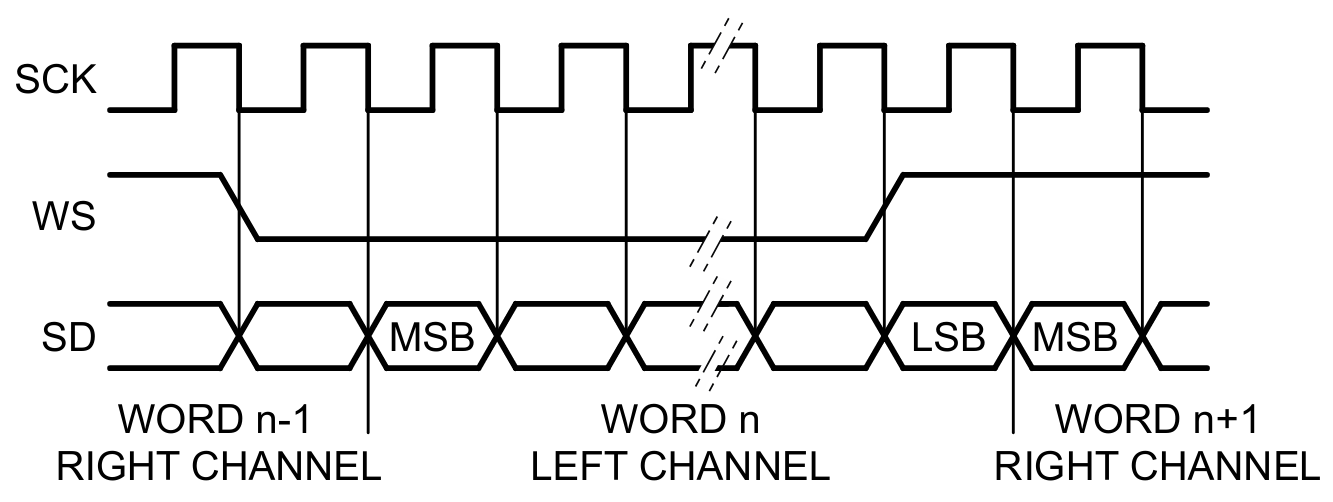
\includegraphics[width=10cm]{img/i2s_timing.png}
    \caption{Timing diagramm of the \ac{I2S} protocol \cite{nxp_i2s}}
    \label{fig:i2s-timing}
\end{figure}

The word length can vary between transmitter and receiver. That is why the \ac{MSB} is sent first in the standard 
configuration. Additionally the participants do not need to know the word length of the counterpart \cite{nxp_i2s}.

The wiring of this serial bus is possible in three basic configurations (shown in \autoref{fig:i2s-config}).
Thereby the master is always responsible for the SCK and the WS line.

\begin{figure}[!h]
    \centering
    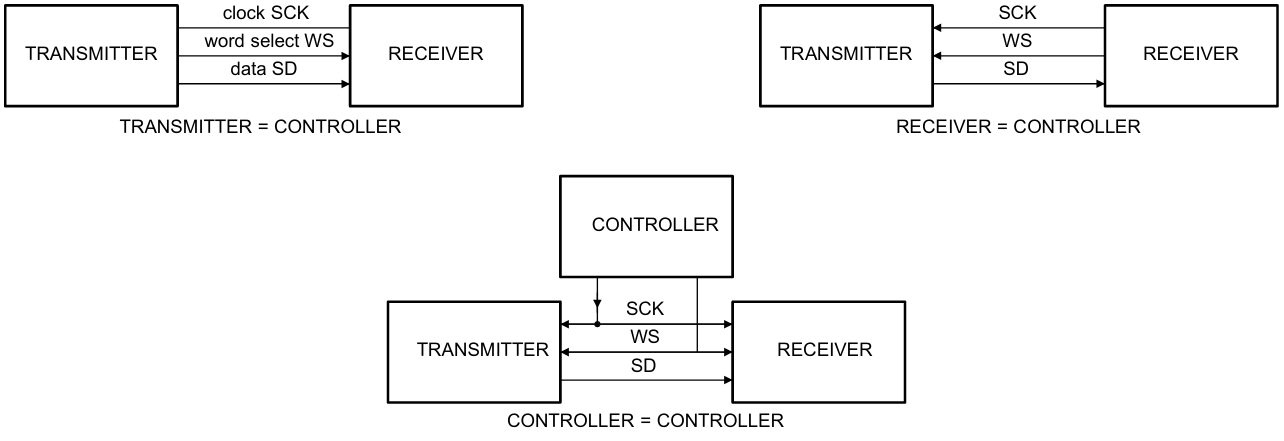
\includegraphics[width=14cm]{img/i2s_config.png}
    \caption{The three basic configurations of the \ac{I2S} protocol \cite{nxp_i2s}}
    \label{fig:i2s-config}
\end{figure}

\subsubsection{Direct Memory Access}
\label{sec:dma}

The \ac{DMA} is a peripheral in the microcontroller, which allows to transfer data between memory destinations or
peripherals without the need of the \ac{CPU}.
This is advantagious, because this saves computation capacity which leads to a smoother data flow.
